\documentclass[aspectratio=169, table, 12pt]{beamer}

% Preamble bersama seluruh slide mata kuliah ini.
% Dipanggil dari slides/sessionXX/sessionXX.tex tepat sesudah baris
% \documentclass[aspectratio=169, table, 12pt]{beamer}
% Paket tambahan yang hanya dibutuhkan satu sesi ditulis di berkas sesi itu.

\usepackage{colortbl}
\usepackage{xcolor}
\usepackage{listings}
\usepackage{tabularx}
\usepackage{booktabs}
\usepackage{tikz}
\usepackage{pgfplots}
\pgfplotsset{compat=1.18}
\usetikzlibrary{arrows.meta, positioning, calc, fit, shapes.geometric,
	shapes.multipart, backgrounds, matrix, chains, trees}

\makeatletter
\def\input@path{{../theme/}}
\makeatother
\graphicspath{{../theme/}{../../figures/}}
\usetheme{Pradita}

\definecolor{praditagreen}{RGB}{37, 113, 71}

% Tema membuat garis tabel berwarna putih. Dikembalikan agar tabel terbaca.
\arrayrulecolor{black}
\setlength{\arrayrulewidth}{0.5pt}

\lstdefinelanguage{yaml}{
	basicstyle=\ttfamily\scriptsize,
	keywordstyle=\color{blue}\bfseries,
	commentstyle=\color{gray}\itshape,
	stringstyle=\color{red},
	showstringspaces=false,
	breaklines=true,
	frame=lines,
	numbers=none,
	backgroundcolor=\color{lightgray!10},
	tabsize=2,
	morecomment=[l]{\#}
}

\lstdefinelanguage{json}{
	basicstyle=\ttfamily\scriptsize,
	stringstyle=\color{red},
	commentstyle=\color{gray},
	breaklines=true,
	showstringspaces=false,
	tabsize=2,
	numbers=none,
	frame=lines,
	backgroundcolor=\color{lightgray!10},
	string=[s]{"}{"}
}

\lstdefinelanguage{bash}{
	keywords={},
	basicstyle=\ttfamily\scriptsize,
	ndkeywords={docker, kubectl, helm, curl, git, terraform},
	ndkeywordstyle=\color{purple}\bfseries,
	sensitive=true,
	commentstyle=\color{gray},
	numbers=none,
	breaklines=true,
	frame=lines,
	backgroundcolor=\color{lightgray!10},
	tabsize=2,
	comment=[l]{\#},
	showstringspaces=false
}

\lstdefinelanguage{http}{
	keywords={GET, POST, PUT, PATCH, DELETE, HEAD, OPTIONS, HTTP},
	basicstyle=\ttfamily\scriptsize,
	keywordstyle=\color{blue}\bfseries,
	sensitive=true,
	numbers=none,
	breaklines=true,
	frame=lines,
	backgroundcolor=\color{lightgray!10},
	tabsize=2,
	showstringspaces=false
}

\subtitle{IT40713 · Cloud-Native \& Microservices Architecture}
\author{\textbf{Alfa Yohannis}}


\title{\Huge Observability,\\ \vspace{10pt} SRE, dan SLO}

\begin{document}

\frame{\titlepage}

\begin{frame}
  \frametitle{Isi Pertemuan}
  \vspace{14pt}
  \begin{columns}[t]
    \column{0.5\textwidth}
    {\small\tableofcontents[sections={1-4}]}

    \column{0.5\textwidth}
    {\small\tableofcontents[sections={5-8}]}
  \end{columns}
\end{frame}

\begin{frame}{\hfill}
  \centering
  \Huge{\textbf{Dasbor hijau,\\pasien gagal memesan.\\Apa yang salah?}}
\end{frame}

\section{Tujuan dan Konteks}

\begin{frame}{\hfill}
  \centering
  \Huge{\textbf{Tujuan dan Konteks}}
\end{frame}

\begin{frame}{{\Large Tujuan Pembelajaran}}
  \vspace{10pt}
  \begin{itemize}
    \item Membedakan \textit{monitoring} dan \textit{observability} serta tiga sinyal
          telemetri: \textit{log}, metrik, dan \textit{trace}.
    \item Menetapkan SLI, SLO, dan \textit{error budget} untuk perjalanan pengguna yang
          kritis.
    \item Menjelaskan praktik SRE (\textit{Site Reliability Engineering}) yang
          menyeimbangkan kecepatan perubahan dan keandalan.
  \end{itemize}
\end{frame}

\begin{frame}{{\Large Dasbor Hijau, Pasien Kecewa}}
  \vspace{10pt}
  \begin{itemize}
    \item Misalkan sepanjang September 2026 semua dasbor hijau: prosesor rata-rata 35
          persen, memori 52 persen.
    \item Pada bulan yang sama: 1.140 keluhan gagal membuat janji temu, terutama ke
          Bandung.
    \item Sekitar 2.300 pemesanan ganda dibatalkan satu per satu.
    \item Dasbor mengukur kondisi mesin, bukan pengalaman pasien.
    \item Ukuran keandalan berangkat dari pertanyaan pasien: berhasil atau tidak, dan
          berapa lama.
  \end{itemize}
\end{frame}

\begin{frame}{{\Large Diagram Konsep Bab 11}}
  \centering
  {\small\bfseries Observabilitas menghubungkan perjalanan pengguna ke keputusan SRE}\par\medskip
  \adjustbox{width=0.96\textwidth,height=0.7\textheight,keepaspectratio}{%
    % Diagram konsep Bab 11: Observabilitas menghubungkan perjalanan pengguna ke keputusan SRE.
% Dibangkitkan tools/render-diagrams.py dari figures/chapter-diagrams.json;
% ubah data JSON lalu jalankan ulang skrip, jangan sunting berkas ini langsung.
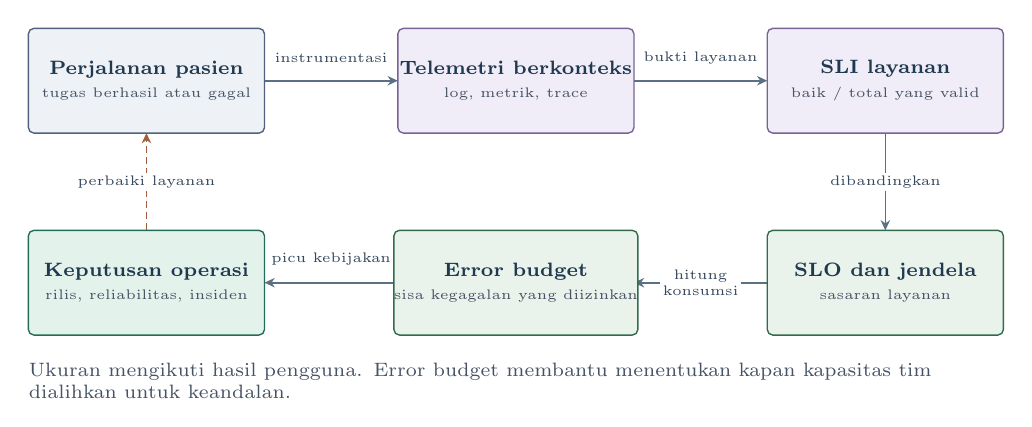
\begin{tikzpicture}[
  x=0.92cm, y=0.95cm,
  kotak konsep/.style={draw, line width=0.5pt, rounded corners=2pt,
    align=center, minimum width=2.999cm,
    minimum height=1.330cm, inner sep=0pt, font=\scriptsize,
    text=konsepJudul},
  peran actor/.style={kotak konsep, fill=konsepIsiActor, draw=konsepGarisActor},
  peran service/.style={kotak konsep, fill=konsepIsiService, draw=konsepGarisService},
  peran control/.style={kotak konsep, fill=konsepIsiControl, draw=konsepGarisControl},
  peran data/.style={kotak konsep, fill=konsepIsiData, draw=konsepGarisData},
  peran outcome/.style={kotak konsep, fill=konsepIsiOutcome, draw=konsepGarisOutcome},
  peran risk/.style={kotak konsep, fill=konsepIsiRisk, draw=konsepGarisRisk},
  panah konsep/.style={-{Stealth[length=1.3mm, width=1.2mm]}, line width=0.6pt,
    draw=konsepPanah},
  panah putus/.style={panah konsep, draw=konsepPanahPutus,
    dash pattern=on 2.5pt off 1.5pt},
  label panah/.style={font=\tiny, align=center, fill=white,
    inner sep=1pt, text=konsepLabel},
  catatan/.style={font=\scriptsize, align=left, anchor=north west,
    inner sep=0pt, text width=12.383cm, text=konsepTeks,
    execute at begin node={\hyphenpenalty=10000\hbadness=10000\relax}},
]
  \definecolor{konsepIsiActor}{HTML}{EEF1F6}
  \definecolor{konsepGarisActor}{HTML}{50627D}
  \definecolor{konsepIsiService}{HTML}{EAF2FB}
  \definecolor{konsepGarisService}{HTML}{3F6893}
  \definecolor{konsepIsiControl}{HTML}{E9F3EC}
  \definecolor{konsepGarisControl}{HTML}{316B4B}
  \definecolor{konsepIsiData}{HTML}{F1EDF8}
  \definecolor{konsepGarisData}{HTML}{786394}
  \definecolor{konsepIsiOutcome}{HTML}{E4F2EC}
  \definecolor{konsepGarisOutcome}{HTML}{236C57}
  \definecolor{konsepIsiRisk}{HTML}{FCEDE7}
  \definecolor{konsepGarisRisk}{HTML}{B36947}
  \definecolor{konsepJudul}{HTML}{20394F}
  \definecolor{konsepTeks}{HTML}{455264}
  \definecolor{konsepLabel}{HTML}{35485C}
  \definecolor{konsepPanah}{HTML}{5C7084}
  \definecolor{konsepPanahPutus}{HTML}{A15D40}
  % Panah dan label lebih dahulu; kotak menutupi sisa latar label.
  \draw[panah konsep] (0.93,0) -- (2.77,0);
  \draw[panah konsep] (6.03,0) -- (7.87,0);
  \draw[panah konsep] (9.5,-0.7) -- (9.5,-2);
  \draw[panah konsep] (7.87,-2.7) -- (6.03,-2.7);
  \draw[panah konsep] (2.77,-2.7) -- (0.93,-2.7);
  \draw[panah putus] (-0.7,-2) -- (-0.7,-0.7);
  \node[label panah] at (1.85,0.31) {instrumentasi};
  \node[label panah] at (6.95,0.31) {bukti layanan};
  \node[label panah] at (9.5,-1.35) {dibandingkan};
  \node[label panah] at (6.95,-2.7) {hitung\\konsumsi};
  \node[label panah] at (1.85,-2.39) {picu kebijakan};
  \node[label panah] at (-0.7,-1.35) {perbaiki layanan};
  \node[peran actor] (journey) at (-0.7,0)
    {\textbf{Perjalanan pasien}\\[0.5pt]{\tiny\color{konsepTeks}tugas berhasil atau gagal}};
  \node[peran data] (tele) at (4.4,0)
    {\textbf{Telemetri berkonteks}\\[0.5pt]{\tiny\color{konsepTeks}log, metrik, trace}};
  \node[peran data] (sli) at (9.5,0)
    {\textbf{SLI layanan}\\[0.5pt]{\tiny\color{konsepTeks}baik / total yang valid}};
  \node[peran outcome] (tindakan) at (-0.7,-2.7)
    {\textbf{Keputusan operasi}\\[0.5pt]{\tiny\color{konsepTeks}rilis, reliabilitas, insiden}};
  \node[peran control] (budget) at (4.4,-2.7)
    {\textbf{Error budget}\\[0.5pt]{\tiny\color{konsepTeks}sisa kegagalan yang diizinkan}};
  \node[peran control] (slo) at (9.5,-2.7)
    {\textbf{SLO dan jendela}\\[0.5pt]{\tiny\color{konsepTeks}sasaran layanan}};
  \node[catatan] at (-2.33,-3.77)
    {Ukuran mengikuti hasil pengguna. Error budget membantu menentukan kapan kapasitas tim dialihkan untuk keandalan.};
\end{tikzpicture}
}
\end{frame}

\section{Monitoring dan Observability}

\begin{frame}{\hfill}
  \centering
  \Huge{\textbf{Monitoring dan\\Observability}}
\end{frame}

\begin{frame}{{\Large Dua Cara Melihat Sistem}}
  \vspace{10pt}
  \begin{itemize}
    \item \textit{Monitoring}: ukuran yang ditentukan sebelumnya, \textit{alert} ketika
          melewati ambang.
    \item \textit{Observability}: menjawab pertanyaan baru dari data yang dikeluarkan
          sistem, tanpa menambah kode lebih dahulu.
    \item Analogi: tanda vital di ruang triase lawan rekam medis lengkap yang dapat
          ditelusuri.
    \item \textit{Observability} tidak menggantikan \textit{monitoring}; keduanya
          dipakai untuk masalah yang berbeda.
  \end{itemize}
\end{frame}

\begin{frame}{{\Large Perbedaan Monitoring dan Observability}}
  \footnotesize
  \begin{tabularx}{\textwidth}{>{\raggedright\arraybackslash}p{2.6cm}
      >{\raggedright\arraybackslash}X >{\raggedright\arraybackslash}X}
    \hline
    \textbf{Aspek} & \textbf{\textit{Monitoring}} & \textbf{\textit{Observability}} \\
    \hline
    Pertanyaan & Sudah ditentukan: apakah ukuran X melewati ambang? & Muncul saat itu:
      mengapa Bandung gagal, Bogor tidak? \\
    \hline
    Paling berguna & Masalah berulang yang sudah dikenal & Masalah baru di sistem dengan
      banyak komponen \\
    \hline
    Contoh Medikara & Prosesor layanan janji temu di atas 80 persen & Kegagalan hanya
      pada pemesanan ke SIMRS Bandung setelah pukul 07.00 \\
    \hline
    Keterbatasan & Buta terhadap masalah yang belum dibayangkan & Telemetri lebih banyak;
      biaya dan perlindungan data dikelola \\
    \hline
  \end{tabularx}
\end{frame}

\begin{frame}{{\Large Mengapa Kebutuhan Ini Makin Terasa}}
  \vspace{6pt}
  \small
  \begin{itemize}
    \item Satu permintaan melintasi lima atau enam layanan milik tim yang berbeda.
    \item Penelusuran 1.140 keluhan butuh 11 hari; dengan nomor penelusuran bersama,
          satu sore.
    \item 312 berkas klaim Depok ``terkirim'' tetapi ditolak; ketahuan 19 hari kemudian,
          sekitar Rp1,7 miliar tertunda.
    \item UU PDP: pemberitahuan tertulis paling lambat 3 kali 24 jam bila pelindungan
          data pribadi gagal.
    \item Telemetri bisa menjadi jalur kebocoran: data pasien tidak ikut dicatat.
  \end{itemize}
\end{frame}

\section{Log, Metrik, dan Trace}

\begin{frame}{\hfill}
  \centering
  \Huge{\textbf{Log, Metrik,\\dan Trace}}
\end{frame}

\begin{frame}{{\Large Tiga Sinyal Telemetri}}
  \footnotesize
  \begin{tabularx}{\textwidth}{>{\raggedright\arraybackslash}p{1.5cm}
      >{\raggedright\arraybackslash}X >{\raggedright\arraybackslash}X
      >{\raggedright\arraybackslash}p{2.6cm}}
    \hline
    \textbf{Sinyal} & \textbf{Pertanyaan} & \textbf{Contoh di Medikara+} &
      \textbf{Biaya simpan} \\
    \hline
    Metrik & Seberapa sering, banyak, dan cepat? & Persentase pemesanan gagal per rumah
      sakit setiap menit & Rendah, sudah diringkas \\
    \hline
    \textit{Log} & Apa yang terjadi pada satu kejadian? & ``Adaptor SIMRS Bandung: batas
      waktu 3 detik habis'' & Tinggi \\
    \hline
    \textit{Trace} & Ke mana satu permintaan pergi, dan di mana waktunya habis? & Satu
      pemesanan melintasi enam komponen dalam 9,8 detik & Tinggi, diambil sampelnya \\
    \hline
  \end{tabularx}

  \vspace{10pt}
  \small
  Analogi: buku gudang (\textit{log}), papan rekap (metrik), dan nomor resi paket
  (\textit{trace}).
\end{frame}

\begin{frame}{{\Large Satu Trace Pemesanan ke Bandung}}
  \centering
  \eadiagram{../../figures/ch11-trace-janji-temu.tex}
\end{frame}

\begin{frame}{{\Large Membaca Trace Itu}}
  \vspace{10pt}
  \begin{itemize}
    \item Total 9,8 detik; layanan jadwal dokter hanya 0,3 detik.
    \item Sekitar 86 persen waktu (8,4 detik) habis di adaptor SIMRS Bandung.
    \item Aplikasi menyerah di detik ke-8; konfirmasi baru terkirim di detik ke-9,5.
    \item Pasien memesan ulang, terjadi pemesanan ganda; prosesor tetap santai.
    \item \textit{Header} \texttt{traceparent} (Trace Context) menyambung \textit{span}
          lintas layanan.
  \end{itemize}
\end{frame}

\begin{frame}{{\Large OpenTelemetry sebagai Standar Terbuka}}
  \vspace{10pt}
  \begin{itemize}
    \item Kerangka sumber terbuka untuk membuat dan mengirim \textit{trace}, metrik, dan
          \textit{log}.
    \item Proyek CNCF yang netral vendor; bukan penyimpanan atau penampil telemetri.
    \item Collector: menerima, menyamarkan data pasien, memilih sampel, meneruskan.
    \item Analogi: colokan listrik standar, peralatan bebas pindah rumah.
    \item Konsekuensi: tidak terkunci vendor; aturan penyamaran ditulis sekali.
  \end{itemize}
\end{frame}

\begin{frame}{{\Large Alur Telemetri Medikara}}
  \centering
  \eadiagram{../../figures/ch11-alur-opentelemetry.tex}
\end{frame}

\begin{frame}{{\Large Biaya Telemetri}}
  \vspace{10pt}
  \begin{itemize}
    \item Empat pengungkit: tingkat \textit{log}, sampel \textit{trace}, masa simpan
          bertingkat, label metrik.
    \item Misalkan 60 GB \textit{log} per hari, Rp7.500 per GB: Rp13,5 juta per bulan.
    \item Setelah dikendalikan: 22 GB per hari, sekitar Rp4,95 juta per bulan.
    \item Nomor rekam medis sebagai label metrik: deret data dari sekitar 300 menjadi
          lebih dari 400.000.
  \end{itemize}
\end{frame}

\section{SLI, SLO, dan SLA}

\begin{frame}{\hfill}
  \centering
  \Huge{\textbf{SLI, SLO,\\dan SLA}}
\end{frame}

\begin{frame}{{\Large Tiga Istilah yang Sering Tertukar}}
  \footnotesize
  \begin{tabularx}{\textwidth}{>{\raggedright\arraybackslash}p{1.2cm}
      >{\raggedright\arraybackslash}X >{\raggedright\arraybackslash}p{2.8cm}
      >{\raggedright\arraybackslash}X}
    \hline
    \textbf{Istilah} & \textbf{Pertanyaan} & \textbf{Penetap} & \textbf{Contoh Medikara} \\
    \hline
    SLI & Seberapa baik layanan saat ini dari sisi pengguna? & Tim teknis dan pemilik
      layanan & Upaya pemesanan terkonfirmasi dalam 5 detik \\
    \hline
    SLO & Seberapa baik seharusnya dalam satu jendela? & Pemilik layanan, disetujui
      manajemen & 99,5 persen dalam 30 hari bergulir \\
    \hline
    SLA & Apa akibatnya bila janji ke pihak luar meleset? & Bisnis dan bagian hukum &
      Misalkan potongan biaya bila di bawah 99 persen \\
    \hline
  \end{tabularx}

  \vspace{10pt}
  \small
  Analogi restoran cepat saji: siap dalam 10 menit (SLI), target dapur 95 persen (SLO),
  minuman gratis bila lewat 15 menit (SLA).
\end{frame}

\begin{frame}{{\Large Memilih SLI dari Perjalanan Pengguna}}
  \footnotesize
  \begin{tabularx}{\textwidth}{>{\raggedright\arraybackslash}p{3.0cm}
      >{\raggedright\arraybackslash}p{2.2cm} >{\raggedright\arraybackslash}X}
    \hline
    \textbf{Jenis layanan} & \textbf{SLI} & \textbf{Peristiwa baik dibagi seluruh peristiwa}
      \\
    \hline
    Menjawab permintaan & Latensi & Pemesanan terkonfirmasi dalam 5 detik \\
    \hline
    Alur pengolahan data & Kesegaran & Hasil laboratorium tampil dalam 30 menit setelah
      divalidasi \\
    \hline
    Alur pengolahan data & Kebenaran & Berkas klaim diterima tanpa penolakan format \\
    \hline
    Penyimpanan & Daya tahan & Dokumen rekam medis terbaca kembali utuh \\
    \hline
  \end{tabularx}

  \vspace{10pt}
  \small
  Halaman hasil laboratorium dapat dibuka 99,97 persen dari waktu, tetapi hanya 91 persen
  hasil tampil dalam 30 menit.
\end{frame}

\begin{frame}{{\Large Waktu Tidak Tersedia yang Diizinkan}}
  \footnotesize
  \begin{tabularx}{\textwidth}{>{\raggedright\arraybackslash}p{2.2cm}
      >{\raggedright\arraybackslash}p{2.4cm} >{\raggedright\arraybackslash}X
      >{\raggedright\arraybackslash}X}
    \hline
    \textbf{Target} & \textbf{\textit{Error budget}} & \textbf{Per 30 hari} &
      \textbf{Per tahun} \\
    \hline
    99 persen & 1 persen & 432 menit & 87 jam 36 menit \\
    \hline
    99,9 persen & 0,1 persen & 43,2 menit & 8 jam 45,6 menit \\
    \hline
    99,95 persen & 0,05 persen & 21,6 menit & 4 jam 22,8 menit \\
    \hline
    99,99 persen & 0,01 persen & 4,32 menit & 52,6 menit \\
    \hline
    99,999 persen & 0,001 persen & sekitar 26 detik & sekitar 5 menit 15 detik \\
    \hline
  \end{tabularx}

  \vspace{10pt}
  \small
  Berbasis permintaan: sekitar 28.000 upaya per 30 hari dengan target 99,5 persen berarti
  140 upaya boleh gagal.
\end{frame}

\begin{frame}{{\Large Mengapa Bukan 100 Persen}}
  \vspace{10pt}
  \begin{itemize}
    \item Pasien tidak dapat membedakan: ponsel dan jaringannya jauh kurang andal.
    \item Biaya naik jauh lebih cepat daripada manfaat setiap tambahan angka sembilan.
    \item Ketergantungan membatasi: adaptor SIMRS hanya ditargetkan 99,5 persen.
    \item \textit{Error budget} nol berarti tidak ada perubahan yang boleh dirilis.
  \end{itemize}
\end{frame}

\begin{frame}{{\Large Kasus Medikara: SLI Tiga Perjalanan Pasien}}
  \footnotesize
  \begin{tabularx}{\textwidth}{>{\raggedright\arraybackslash}p{2.6cm}
      >{\raggedright\arraybackslash}X >{\raggedright\arraybackslash}p{1.2cm}
      >{\raggedright\arraybackslash}p{2.8cm}}
    \hline
    \textbf{Perjalanan} & \textbf{SLI} & \textbf{SLO} & \textbf{\textit{Error budget}} \\
    \hline
    Membuat janji temu & Upaya terkonfirmasi dalam 5 detik & 99,5\% & 140 dari sekitar
      28.000 upaya \\
    \hline
    Hasil laboratorium & Hasil tampil dalam 30 menit setelah divalidasi & 99,0\% & 620 dari
      sekitar 62.000 hasil \\
    \hline
    Klaim BPJS Kesehatan & Berkas diterima tanpa penolakan format dalam 2 hari kerja &
      98,0\% & 820 dari sekitar 41.000 berkas \\
    \hline
  \end{tabularx}

  \vspace{10pt}
  \small
  Usulan 99,9 persen ditolak: dua zona dan petugas jaga 24 jam, biaya kira-kira dua kali
  lipat.
\end{frame}

\section{Error Budget}

\begin{frame}{\hfill}
  \centering
  \Huge{\textbf{Error Budget}}
\end{frame}

\begin{frame}{{\Large Error Budget dan Laju Pembakaran}}
  \vspace{10pt}
  \small
  \begin{itemize}
    \item \textit{Error budget} adalah 100 persen dikurangi target SLO.
    \item Pemesanan Medikara+: target 99,5 persen dari sekitar 28.000 upaya, jadi 140
          upaya boleh gagal per 30 hari.
    \item Analogi: kuota data seluler bulanan; boleh dipakai, tetapi diawasi.
    \item Laju pembakaran 1: habis tepat di hari ke-30; laju 2: habis di hari ke-15.
    \item Jam biasa sekitar 39 upaya, 7,2 persen gagal: laju 14,4, anggaran habis dalam 50 jam.
  \end{itemize}
\end{frame}

\begin{frame}{{\Large Sisa Anggaran dalam Satu Jendela}}
  \centering
  \eadiagram{../../figures/ch11-sisa-anggaran.tex}
\end{frame}

\begin{frame}{{\Large Kebijakan Error Budget Medikara}}
  \footnotesize
  \begin{tabularx}{\textwidth}{>{\raggedright\arraybackslash}p{2.6cm}
      >{\raggedright\arraybackslash}p{2.4cm} >{\raggedright\arraybackslash}X
      >{\raggedright\arraybackslash}p{2.6cm}}
    \hline
    \textbf{Sisa anggaran} & \textbf{Status} & \textbf{Tindakan} & \textbf{Pemutus} \\
    \hline
    Di atas 50\% & Normal & Rilis seperti biasa & Tim pemilik \\
    \hline
    25 sampai 50\% & Waspada & Rilis berisiko besar ditinjau dulu & Pemimpin teknis \\
    \hline
    Di bawah 25\% & Fokus keandalan & Hanya keandalan, keamanan, keselamatan pasien &
      Pemimpin teknis \\
    \hline
    Habis & Beku & Rilis fitur berhenti sampai SLI di atas SLO & Direktur TI \\
    \hline
  \end{tabularx}

  \vspace{10pt}
  \small
  Alat negosiasi: fitur pembayaran digeser ke Desember karena sisa anggaran tinggal 22
  persen.
\end{frame}

\section{Praktik SRE}

\begin{frame}{\hfill}
  \centering
  \Huge{\textbf{Praktik SRE}}
\end{frame}

\begin{frame}{{\Large Toil dan Batasnya}}
  \vspace{10pt}
  \small
  \begin{itemize}
    \item \textit{Toil}: manual, berulang, dapat diotomasi, taktis, tanpa nilai jangka
          panjang, tumbuh seiring layanan.
    \item Batas Google: pekerjaan operasi di bawah 50 persen waktu insinyur SRE.
    \item Menyalakan ulang adaptor SIMRS di 5 rumah sakit: 100 menit per hari, sekitar 50
          jam per bulan.
    \item Laporan ketersediaan dari tangkapan layar: enam hari kerja per bulan.
    \item Analogi: menyalin lima laporan setiap pagi lawan membuat laporan otomatis sekali.
  \end{itemize}
\end{frame}

\begin{frame}{{\Large Alerting Berbasis Laju Pembakaran}}
  \footnotesize
  \begin{tabularx}{\textwidth}{>{\raggedright\arraybackslash}p{2.4cm}
      >{\raggedright\arraybackslash}p{2.2cm} >{\raggedright\arraybackslash}p{2.2cm}
      >{\raggedright\arraybackslash}p{1.6cm} >{\raggedright\arraybackslash}X}
    \hline
    \textbf{Anggaran terpakai} & \textbf{Jendela panjang} & \textbf{Jendela pendek} &
      \textbf{Laju} & \textbf{Pemberitahuan} \\
    \hline
    2 persen & 1 jam & 5 menit & 14,4 & Panggil petugas jaga \\
    \hline
    5 persen & 6 jam & 30 menit & 6 & Panggil petugas jaga \\
    \hline
    10 persen & 3 hari & 6 jam & 1 & Tiket jam kerja \\
    \hline
  \end{tabularx}

  \vspace{10pt}
  \small
  \begin{itemize}
    \item Syarat: mendesak, dapat ditindaklanjuti, butuh pertimbangan manusia.
    \item Medikara: dari sekitar 300 \textit{alert} per minggu menjadi rata-rata empat
          panggilan per bulan.
  \end{itemize}
\end{frame}

\begin{frame}{{\Large Penanganan Insiden}}
  \centering
  \eadiagram{../../figures/ch11-alur-insiden.tex}
\end{frame}

\begin{frame}{{\Large Postmortem dan Pelaporan}}
  \vspace{10pt}
  \small
  \begin{itemize}
    \item \textit{Postmortem} tanpa menyalahkan: fokus pada sistem dan proses, bukan
          individu.
    \item Isi: ringkasan, dampak dan anggaran terpakai, linimasa, penyebab, tindak lanjut
          berpemilik.
    \item Analogi: penyelidikan kecelakaan penerbangan mencegah terulang, bukan menghukum.
    \item Direksi: keberhasilan perjalanan kritis, sisa anggaran berwarna, status tindak
          lanjut, tren.
    \item KPI dan format laporan direksi dibahas rinci di IT40813.
  \end{itemize}
\end{frame}

\begin{frame}{{\Large Kasus Medikara: Postmortem Vaksinasi}}
  \vspace{6pt}
  \small
  \begin{itemize}
    \item 09.00 notifikasi ke semua pengguna; 09.20 sekitar 9.600 pengguna, respons 14
          detik.
    \item 09.27 pusat layanan pelanggan melapor: deteksi pertama datang dari manusia.
    \item Sekitar 1.380 dari 6.000 upaya gagal: hampir sepuluh kali anggaran 30 hari.
    \item Faktor: penskalaan vertikal, sesi di memori, menyala 11 menit, notifikasi
          serentak, \textit{alert} prosesor.
    \item Tindak lanjut: notifikasi bertahap, \textit{alert} laju pembakaran, sesi
          bersama, kalender kampanye.
  \end{itemize}
\end{frame}

\section{Aktivitas}

\begin{frame}{{\Large Aktivitas: SLO Layanan Kritis}}
  \vspace{6pt}
  \small
  \begin{enumerate}
    \item Pilih dua sampai tiga perjalanan pengguna yang kritis.
    \item Rumuskan SLI sebagai rasio peristiwa baik dibagi seluruh peristiwa.
    \item Tetapkan SLO dan hitung \textit{error budget} dalam menit dan permintaan.
    \item Daftar sinyal telemetri; tandai data pribadi yang tidak boleh dicatat.
    \item Tulis kebijakan \textit{error budget} satu halaman.
  \end{enumerate}
\end{frame}

\begin{frame}{{\Large Aktivitas: Peran dan Luaran}}
  \vspace{6pt}
  \small
  \begin{itemize}
    \item Anggota non-teknis: arti ``layanan yang baik'' bagi pasien dan manajemen.
    \item Anggota teknis: SLI, target SLO, titik ukur, dan kebutuhan telemetri.
    \item Seluruh tim: kebijakan \textit{error budget} dan pengambil keputusannya.
    \item Luaran C3: tabel SLO, alur telemetri, dan kebijakan satu halaman.
    \item Berkas: \berkas{sources/chapter11/}, termasuk contoh OpenTelemetry opsional.
  \end{itemize}
\end{frame}

\section{Ringkasan dan Latihan}

\begin{frame}{{\Large Ringkasan}}
  \vspace{6pt}
  \small
  \begin{itemize}
    \item Dasbor hijau belum menjamin pasien terlayani.
    \item Metrik, \textit{log}, dan \textit{trace} saling melengkapi; OpenTelemetry
          menyediakannya secara baku.
    \item SLI diukur dari sisi pengguna; SLO menetapkan target; SLA menambah konsekuensi.
    \item \textit{Error budget} mengubah target menjadi anggaran yang dapat dibelanjakan.
    \item Keandalan diukur dari pengalaman pasien dan ditargetkan secukupnya.
  \end{itemize}
\end{frame}

\begin{frame}{{\Large Latihan}}
  \vspace{6pt}
  \small
  \begin{enumerate}
    \item Hitung waktu tidak tersedia yang diizinkan dalam satu bulan untuk SLO
          ketersediaan 99,5 persen dan 99,9 persen. Jelaskan dampak selisihnya bagi biaya.
    \item Mengapa target SLO 100 persen hampir selalu merupakan keputusan yang buruk?
    \item Usulkan satu SLI untuk layanan janji temu yang mencerminkan pengalaman pasien,
          bukan sekadar kondisi \textit{server}.
  \end{enumerate}
\end{frame}

\end{document}
